\section{System Design}\label{sec:4}

We describe \JobMatch by the user needs it addresses, the components that address them, and the boundaries between them.
The system is organized as three cooperating interaction components, each with a single user constituency and a clearly defined interface to the others.
The data structures and algorithms are documented in the supplementary material; the focus here is the division of responsibility from the user's point of view.

\leadpara{Overview}
\leadpara{C1: Candidate-side component.}
The candidate-side component maintains a structured representation of what the job seeker has told the system about themselves.
It accepts a resume, parses it into discrete fields, normalizes the field values against a shared vocabulary, and presents the parsed result to the user as a review form.
Only after the user confirms a save does the component register a versioned snapshot and emit a snapshot event to the matchmaking component.
The component does not see job descriptions, does not call the matchmaking component directly, and does not act on the user's behalf.
\figref{fig:candidate-pipeline} shows the ingestion and representation pipeline; the user-facing surface is the review form, and the back-end store is the in-memory profile registry that backs the snapshot.

\leadpara{C2: Employer-side component.}
The employer-side component plays the symmetric role for hiring organizations.
It accepts a job description, parses it into required and preferred skills, experience bounds, compensation band, remote policy, and descriptive text, and presents the parsed result to a recruiter as a review form.
Only on confirmation does it register a versioned snapshot.
The component does not see candidate profiles and does not write to the matchmaking component's store.
\figref{fig:employer-pipeline} shows the symmetric ingestion and representation pipeline; the user-facing surface is the recruiter review form, and the back-end store is the in-memory job registry.

\leadpara{C3: Matchmaking component.}
The matchmaking component reads candidate and job snapshots by identifier, scores each feasible pair using a configured strategy, attaches component-level reasons, attaches a calibrated confidence value, and returns the ranked list.
It never writes into a candidate or job store; it never calls C1 or C2 directly; it never acts on behalf of either side.
When a snapshot event arrives, it drops cached rankings that depend on the changed entity and recomputes on the next request.
\figref{fig:matchmaking-workflow} shows the end-to-end matchmaking workflow: ingestion, snapshot, ranking, optional coach feedback, and user actions.

This three-component layout is, in the language of the prior submission, a multi-agent system; the difference in the present framing is the description of each component by the user need it addresses, the information it returns, and the control it preserves, rather than by its internal data flow.
\figref{fig:arch} shows the high-level layout; \figref{fig:workflows} traces the end-to-end flows for both sides.

\begin{figure}[!htbp]
\centering
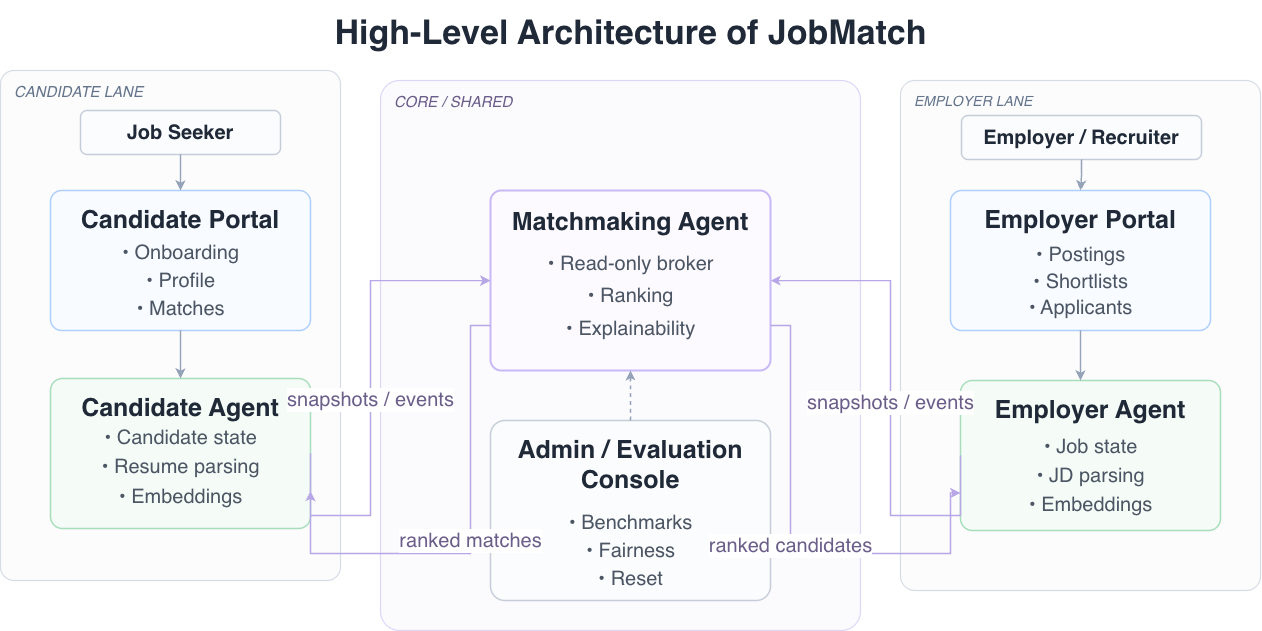
\includegraphics[width=0.95\linewidth]{../figures/Fig1.png}
\caption{High-level layout of \JobMatch. The candidate-side component (C1) and the employer-side component (C2) own the user-editable state on each side of the market. The matchmaking component (C3) reads those snapshots, returns a ranked list with component-level reasons and a calibrated confidence, and never writes into either store. The dashed arrows represent snapshot and event flow; the solid arrows represent user-facing recommendations and feedback.}
\label{fig:arch}
\end{figure}

\begin{figure}[!htbp]
\centering
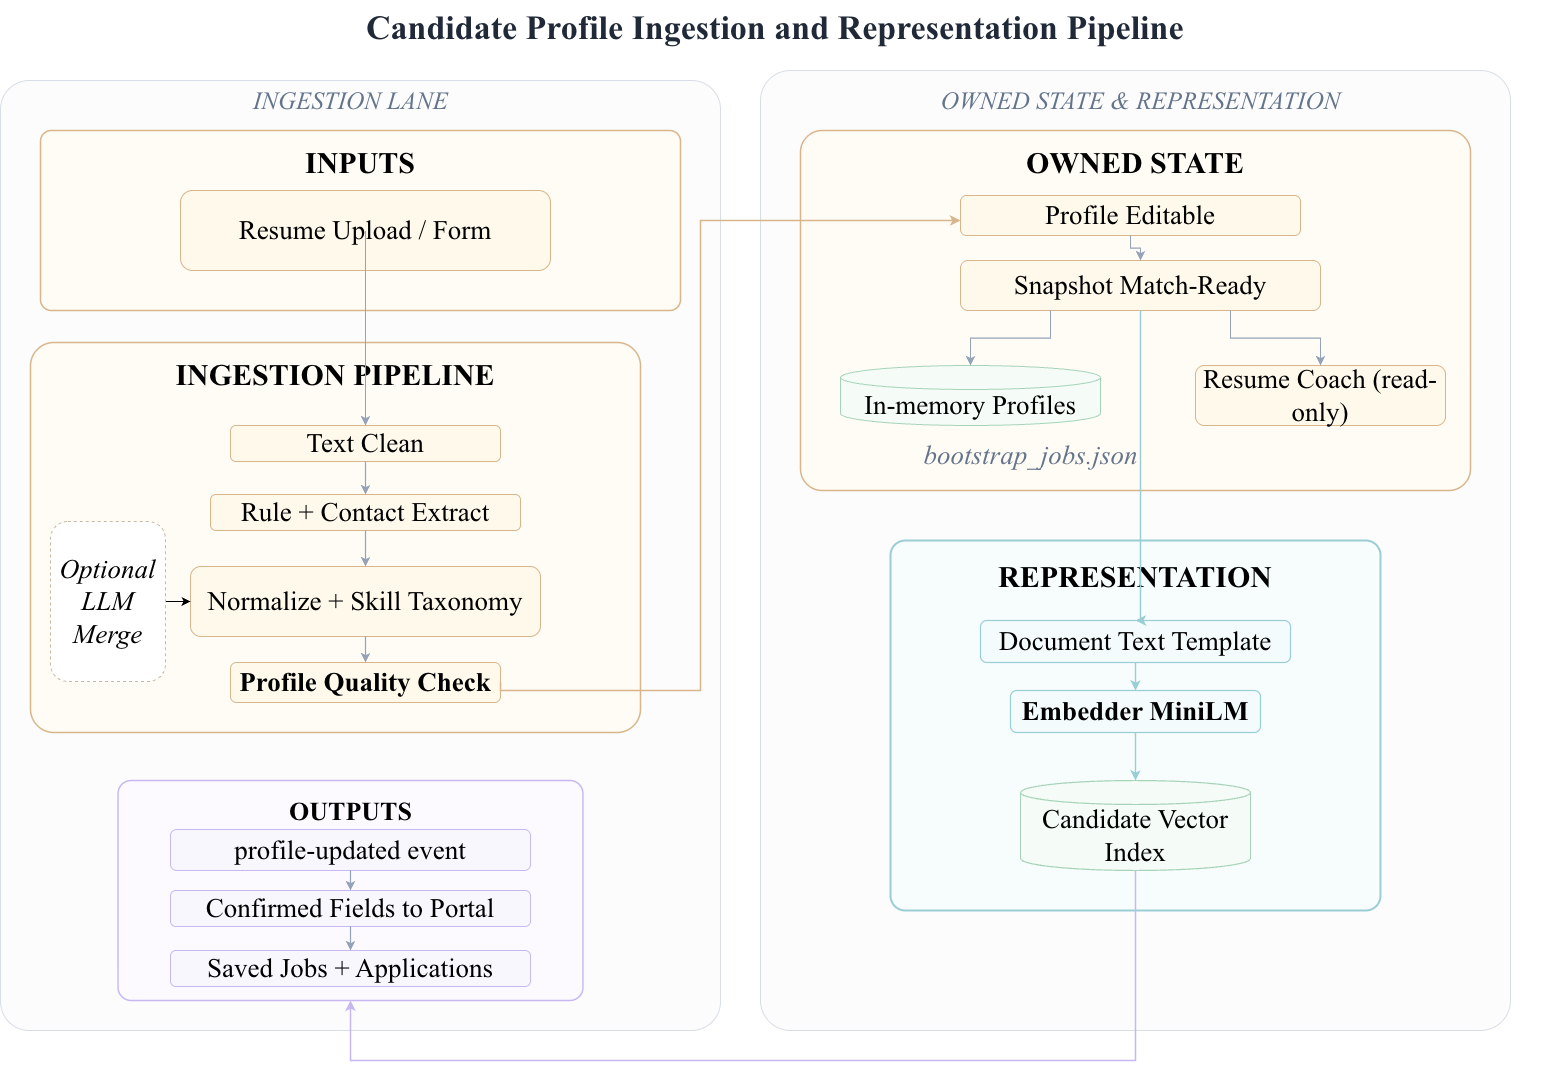
\includegraphics[width=0.95\linewidth]{../figures/Fig2.png}
\caption{Candidate-side ingestion and representation pipeline. The candidate-side component owns the editable profile and the versioned snapshot. The ingestion lane accepts a resume upload, runs text clean and rule-based extraction, normalizes the result against the shared skill vocabulary (with an optional LLM fallback for ambiguous fields), and presents the parsed result to the user as a review form. Only on user confirmation does the component register a snapshot and emit a profile-updated event.}
\label{fig:candidate-pipeline}
\end{figure}

\begin{figure}[!htbp]
\centering
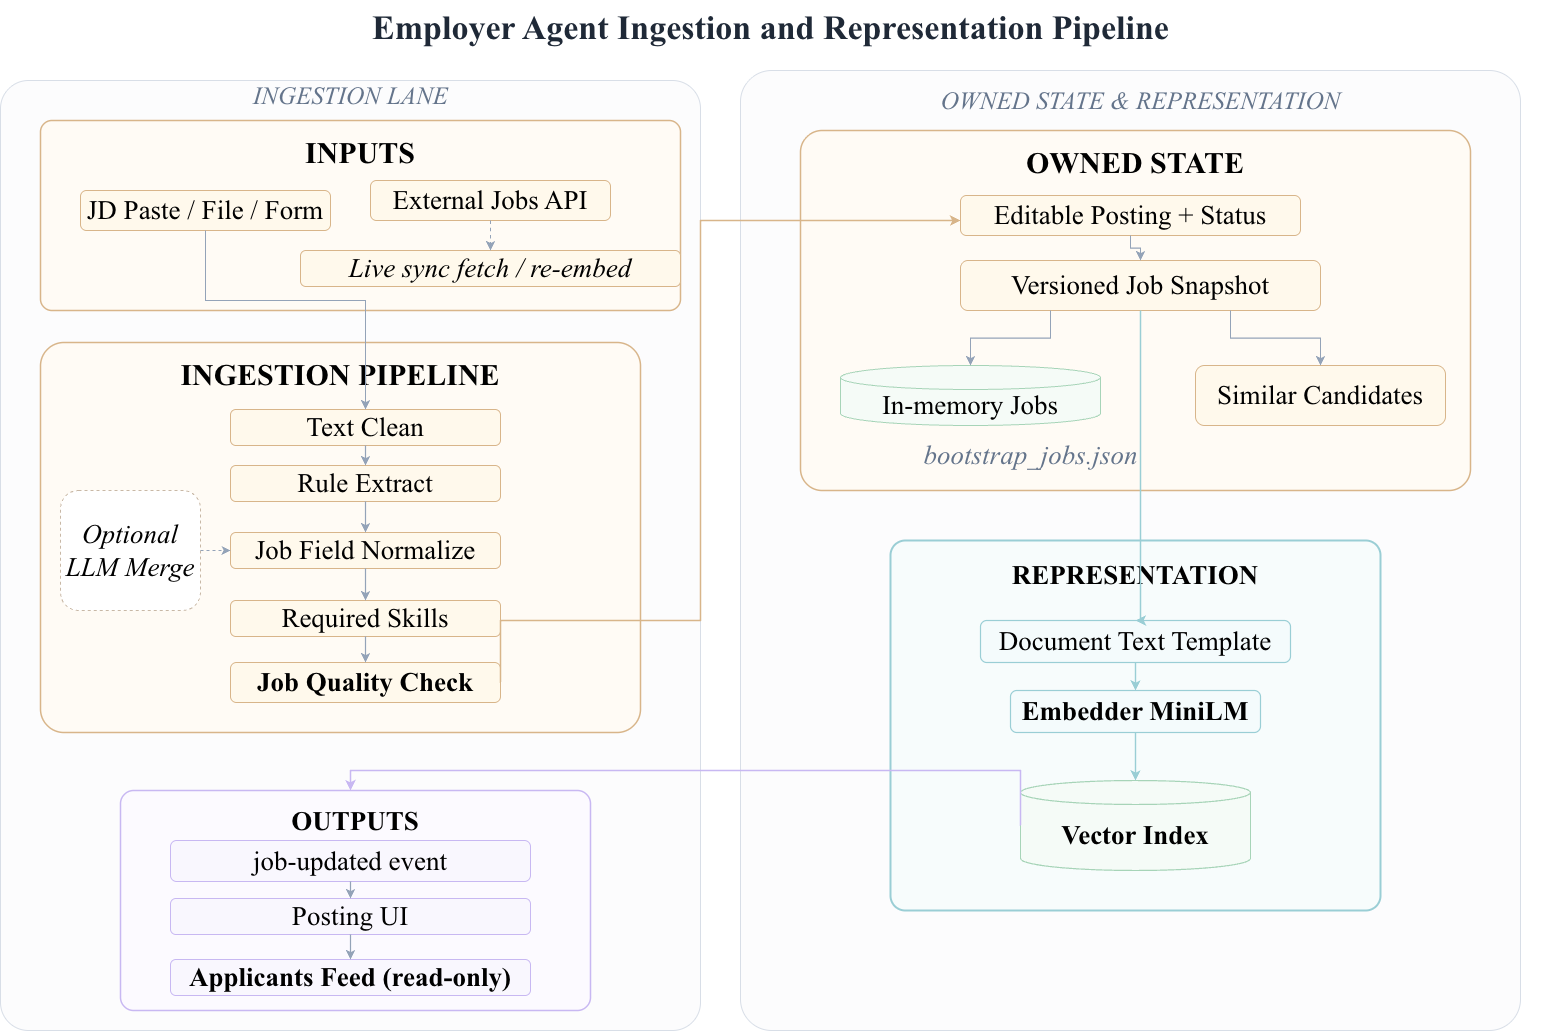
\includegraphics[width=0.95\linewidth]{../figures/Fig3.png}
\caption{Employer-side ingestion and representation pipeline. The employer-side component mirrors the candidate-side layout for the job side: editable posting, versioned snapshot, and an ingestion lane that accepts a job description paste, file, or external API and presents the parsed result as a recruiter review form. Only on confirmation does the component register a snapshot and emit a job-updated event.}
\label{fig:employer-pipeline}
\end{figure}

\begin{figure}[!htbp]
\centering
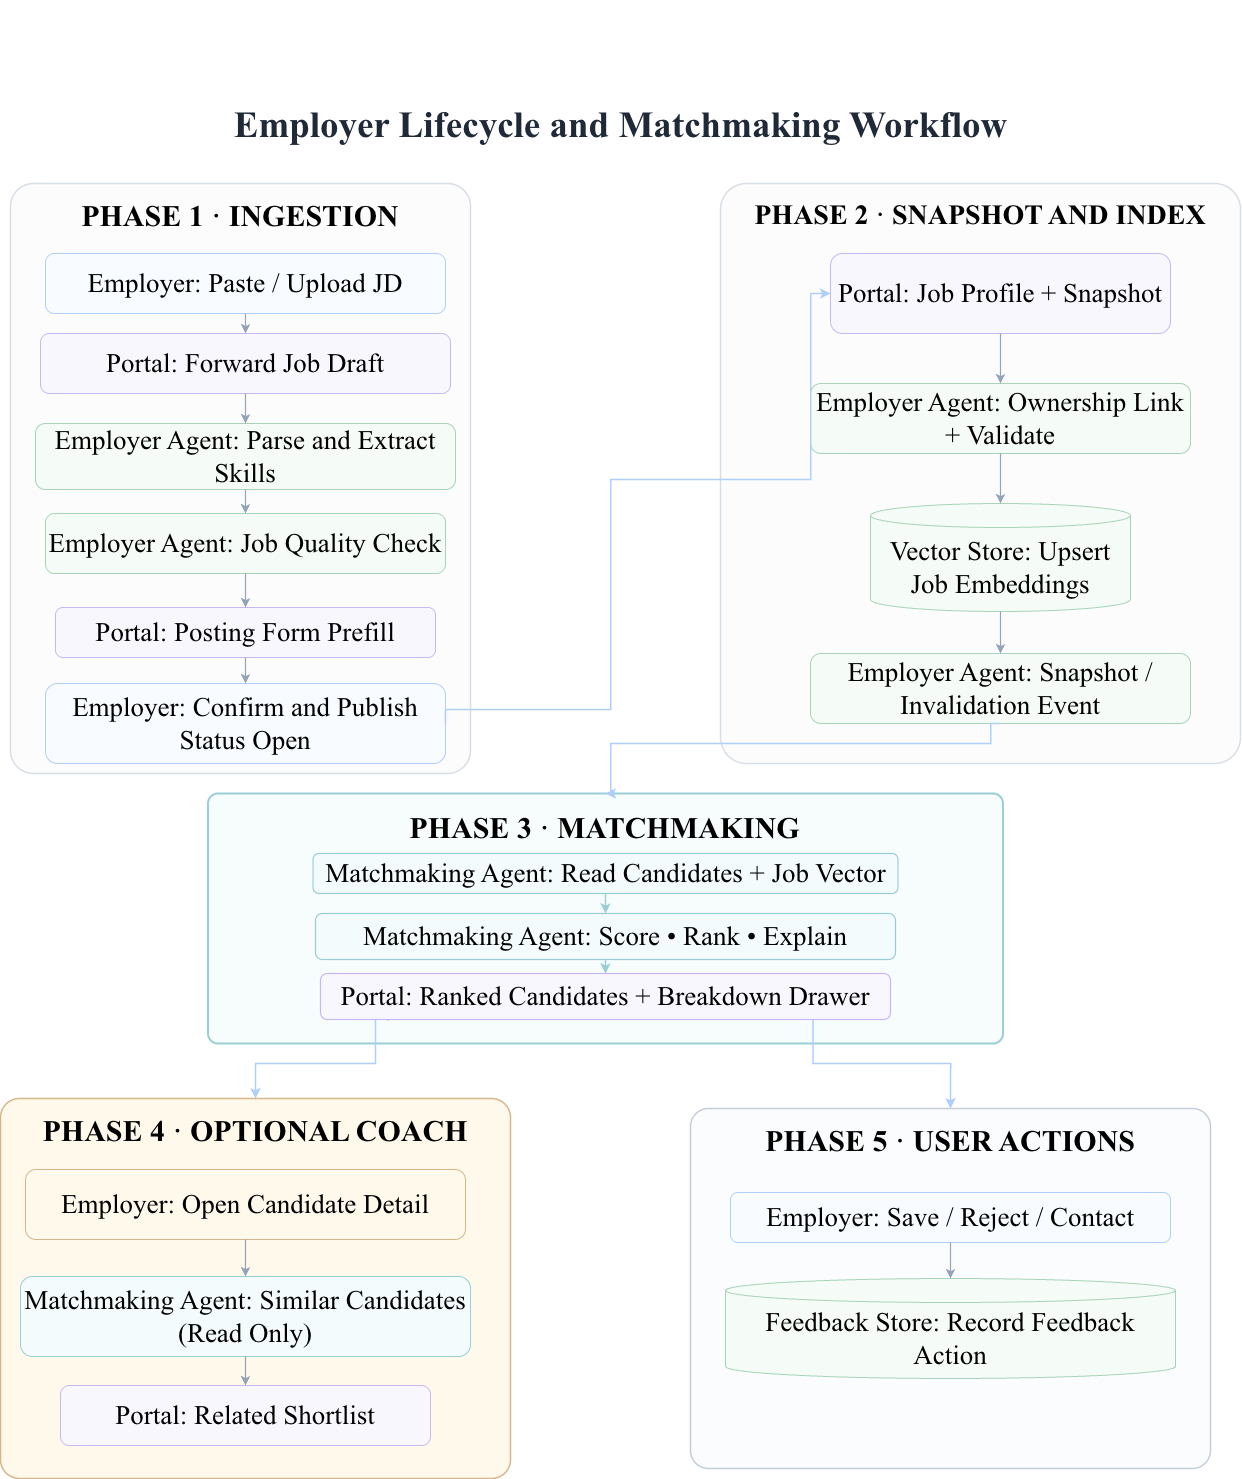
\includegraphics[width=0.95\linewidth]{../figures/Fig4.png}
\caption{End-to-end matchmaking workflow. Ingestion, snapshot/index, ranking, optional coach feedback, and user actions are sequenced so the read-only matchmaking component never crosses the ownership boundary. The workflow is the same whether it is initiated by a candidate refreshing their matches or by an employer refreshing their shortlist.}
\label{fig:matchmaking-workflow}
\end{figure}

\begin{figure}[!htbp]
\centering
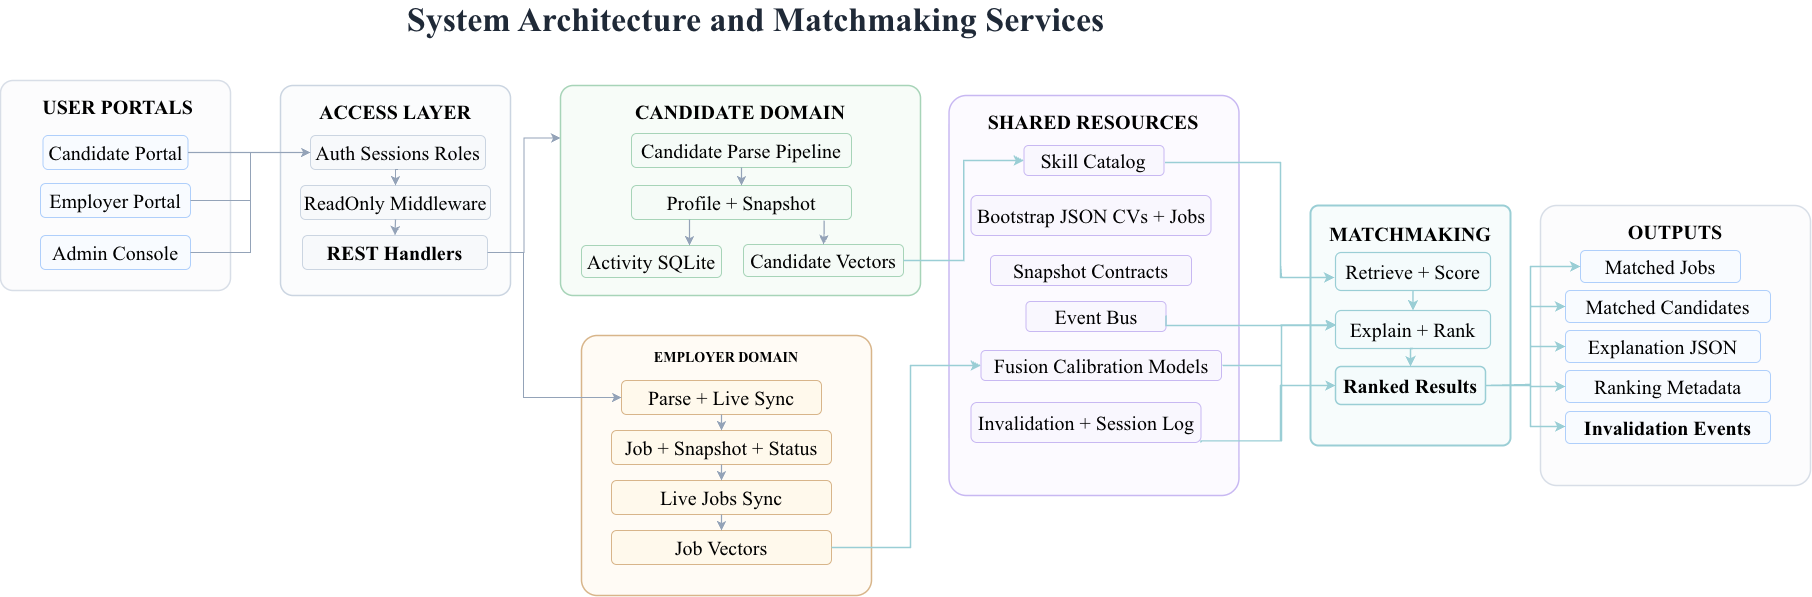
\includegraphics[width=0.95\linewidth]{../figures/Fig7.png}
\caption{Detailed view of the same layout with each lane expanded. The candidate lane shows the job seeker, the candidate portal, and the candidate-side component; the employer lane shows the recruiter, the employer portal, and the employer-side component. The matchmaking component sits in the middle as a read-only broker. An admin/evaluation console provides inspection without crossing ownership boundaries.}
\label{fig:workflows}
\end{figure}

\leadpara{What each component provides to the user}
\emph{C1 (candidate-side).}
\emph{User need:} a job seeker who has edited a resume should be able to verify what the system now knows about them and to revise it before the next recommendation.
\emph{Information provided:} parsed fields, normalized skills, a confidence flag for each field, the version of the snapshot currently in use, and a side-by-side view of the editable profile and the snapshot.
\emph{Control preserved:} the snapshot is updated only on user confirmation; the user can edit any parsed field; the user can revert to a previous snapshot.
\emph{Contribution to explanation:} the candidate-side component is the source of every field the matchmaking component names in an explanation, so a candidate who reads a low score on a remote-policy component can locate the remote-policy field in the snapshot and revise it.

\emph{C2 (employer-side).}
\emph{User need:} a recruiter who has revised a job description should be able to verify which requirements the system now considers and to revise them before the next shortlist.
\emph{Information provided:} required and preferred skills, experience bounds, compensation band, remote policy, descriptive text, the version of the snapshot currently in use, and a flag for each requirement that indicates whether it currently constrains the ranking.
\emph{Control preserved:} the snapshot is updated only on user confirmation; the user can toggle a requirement between required and preferred; the user can revert to a previous snapshot.
\emph{Contribution to explanation:} the employer-side component is the source of every requirement the matchmaking component names in a shortlist explanation.

\emph{C3 (matchmaking).}
\emph{User need:} a user (candidate or recruiter) who has just confirmed a snapshot should be able to read, in the same interaction, what the system ranked and why, with enough detail to decide whether to act.
\emph{Information provided:} a ranked list, a component-level reason for each list item, a calibrated confidence value, a small set of counterfactual edits that would move the item, and an action menu that exposes apply, save, dismiss, and (on the employer side) shortlist and contact.
\emph{Control preserved:} the matchmaking component never acts on the user's behalf; the user can dismiss an item, ask the component to re-rank with a constraint, or close the interaction without further action.
\emph{Contribution to explanation:} the matchmaking component is the only component that aggregates the snapshot channels, so it is the natural place to expose the per-channel contributions and the calibrated confidence.

\leadpara{Communication and state sharing}
The three components exchange two kinds of artifacts.
\emph{Snapshots} cross the boundary from C1 and C2 to C3 as read-only data; the matchmaking component never sees the editable profile behind a snapshot, and C1 and C2 never see each other's state.
\emph{Events} flow back from C1 and C2 to C3 when a snapshot is confirmed or reverted; they carry no editable content, only an identifier and a version.
This division of labor has three consequences we rely on elsewhere in the paper.
First, an explanation in the user interface is bound to the snapshot that produced it, so a user who reverts to a previous snapshot will see explanations based on that previous snapshot.
Second, a recruiter cannot directly inspect a candidate's editable profile, and a candidate cannot directly inspect a recruiter's editable job description, even if both see the same match score; the privacy boundary coincides with the ownership boundary.
Third, an administrator can inspect the matchmaking component's behavior, the candidate-side component's behavior, and the employer-side component's behavior independently, which is what makes the evaluation in \secref{sec:7} tractable.

\leadpara{From components to interaction patterns}
The components above are not the user-facing contribution of the paper; the user-facing contribution is the set of interaction patterns the components enable.
The next section walks through those interaction patterns in the order a user encounters them.
